%-------------------3.1
\subsection{\hll{Code listing using \xmyboxg{minted} in \xmyboxg{beamer}}}
\begin{table}[h!]
\begin{tabular}{c | c}
\begin{minipage}[m]{0.4\textwidth}
\enum{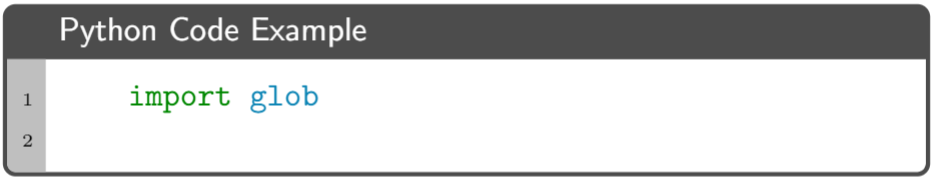
\includegraphics[width=1\linewidth]{3.1.png}}{3.1}
\end{minipage}
&
\begin{minipage}[m]{0.55\textwidth}
\renewcommand\textminus{\mbox{-}}%<<<<<<<<<<<
\begin{lstlisting}[numberstyle=\zebra{pink!15}{green!15},numbers=left,basicstyle=\ttfamily\footnotesize]{tex}
\documentclass{beamer}
\usepackage{tcolorbox}
\tcbuselibrary{minted,skins,breakable}
\newtcblisting{pythoncode}[2][]{
  listing engine=minted, breakable,  colback=bg,
  colframe=black!70,  listing only,
  minted style=colorful,  minted language=python,
  minted options={numbersep=3mm,texcl=true,#1},
  left=5mm,enhanced,
  overlay={\begin{tcbclipinterior}\fill[black!25] (frame.south west)
rectangle ([xshift=5mm]frame.north west);\end{tcbclipinterior}},
#2,}
\begin{document}
\begin{frame}[fragile]
    \frametitle{Premature Optimization}
    \begin{pythoncode}[linenos=true,]{title=Python Code Example}
    import glob
    \end{pythoncode}
\end{frame}
\end{document}
\end{lstlisting}
\end{minipage}
\end{tabular}
\end{table}

%-------------------3.2
\subsection{\hll{"Zebra" style listing}}
\begin{table}[h!]
\begin{tabular}{c | c}
\begin{minipage}[m]{0.4\textwidth}
 \begin{lstlisting}[numberstyle=\zebra{green!25}{yellow!25},numbers=left,basicstyle=\ttfamily\footnotesize]
/**
* Prints Hello World.
**/
#include <stdio.h>

int main(void) {
   printf("Hello World!");
   return 0;
}
\end{lstlisting} 
\end{minipage}
&
\begin{minipage}[m]{0.55\textwidth}
\renewcommand\textminus{\mbox{-}}%<<<<<<<<<<<
\begin{tiny}
\begin{verbatim}
\documentclass{article}
\usepackage[T1]{fontenc}
\usepackage{beramono}
\usepackage{listings}
\usepackage{xcolor}
\newcommand\realnumberstyle[1]{}
\makeatletter
\newcommand{\zebra}[3]{%
    {\realnumberstyle{#3}}%
    \begingroup
    \lst@basicstyle
    \ifodd\value{lstnumber}%
        \color{#1}%
    \else
        \color{#2}%
    \fi
        \rlap{\hspace*{\lst@numbersep}%
        \color@block{\linewidth}{\ht\strutbox}{\dp\strutbox}%
        }%
    \endgroup}
\makeatother
\begin{document}
\begin{lstlisting}[language=C,basicstyle=\ttfamily,
numberstyle=\zebra{green!35}{yellow!35},numbers=left]
/**
* Prints Hello World.
**/
#include <stdio.h>
int main(void) {
   printf("Hello World!");
   return 0;
}
\end{lstlisting}
\end{document}
\end{verbatim}
\end{tiny}
\end{minipage}
\end{tabular}
\end{table}
\clearpage

%-------------------3.3

\subsection{\hll{Listing with russian language}}
\begin{table}[h!]
\begin{tabular}{c | c}
\begin{minipage}[m]{0.4\textwidth}
\enum{ 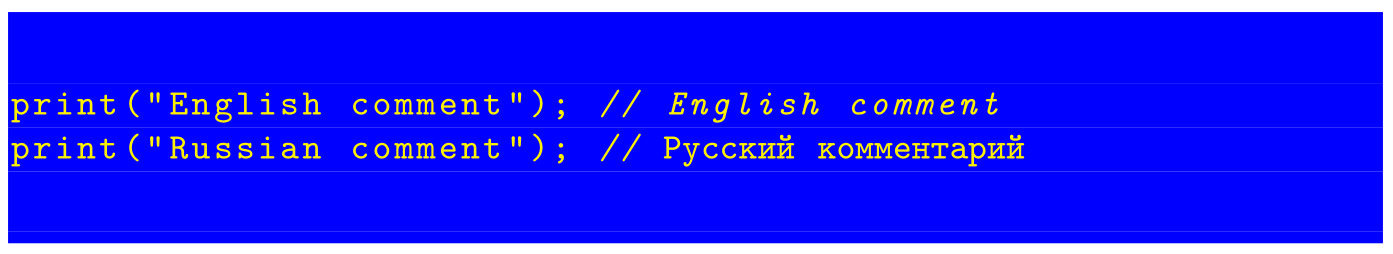
\includegraphics[width=1\linewidth]{3.3.png} }{3.3}
\end{minipage}
&
\begin{minipage}[m]{0.55\textwidth}
\renewcommand\textminus{\mbox{-}}%<<<<<<<<<<<
\begin{lstlisting}[numberstyle=\zebra{pink!15}{green!15},numbers=left,basicstyle=\ttfamily\footnotesize] 
\documentclass{article}
\usepackage[T2A]{fontenc}
\usepackage[utf8]{inputenc}
\usepackage[russian]{babel}
\usepackage{listings} 
\usepackage{xcolor}

\begin{document}
\lstset{ keepspaces=true, 
backgroundcolor=\color{blue},  
showstringspaces=false, 
language=C, 
extendedchars=\true, 
framexrightmargin=0pt,
framexleftmargin=0pt,
framextopmargin=15pt,
framexbottommargin=15pt, 
frame=tb, framerule=0pt,
basicstyle=\color{yellow}\ttfamily\small}

begin{lstlisting}% <<<<<<<<< add "/"
print("English comment"); // English comment
print("Russian comment"); // %here can be russian words
end{lstlisting}%   <<<<<<<<< add "/"
\end{document}
\end{lstlisting}
\end{minipage}
\end{tabular}
\end{table}
 
%-------------------3.4
\subsection{\hll{Listing with \xmyboxg{minted}}}
\begin{table}[h!]
\begin{tabular}{c | c}
\begin{minipage}[m]{0.4\textwidth}
\enum{ \href{https://tex.stackexchange.com/questions/174455/typeset-source-code-with-tcolorbox}{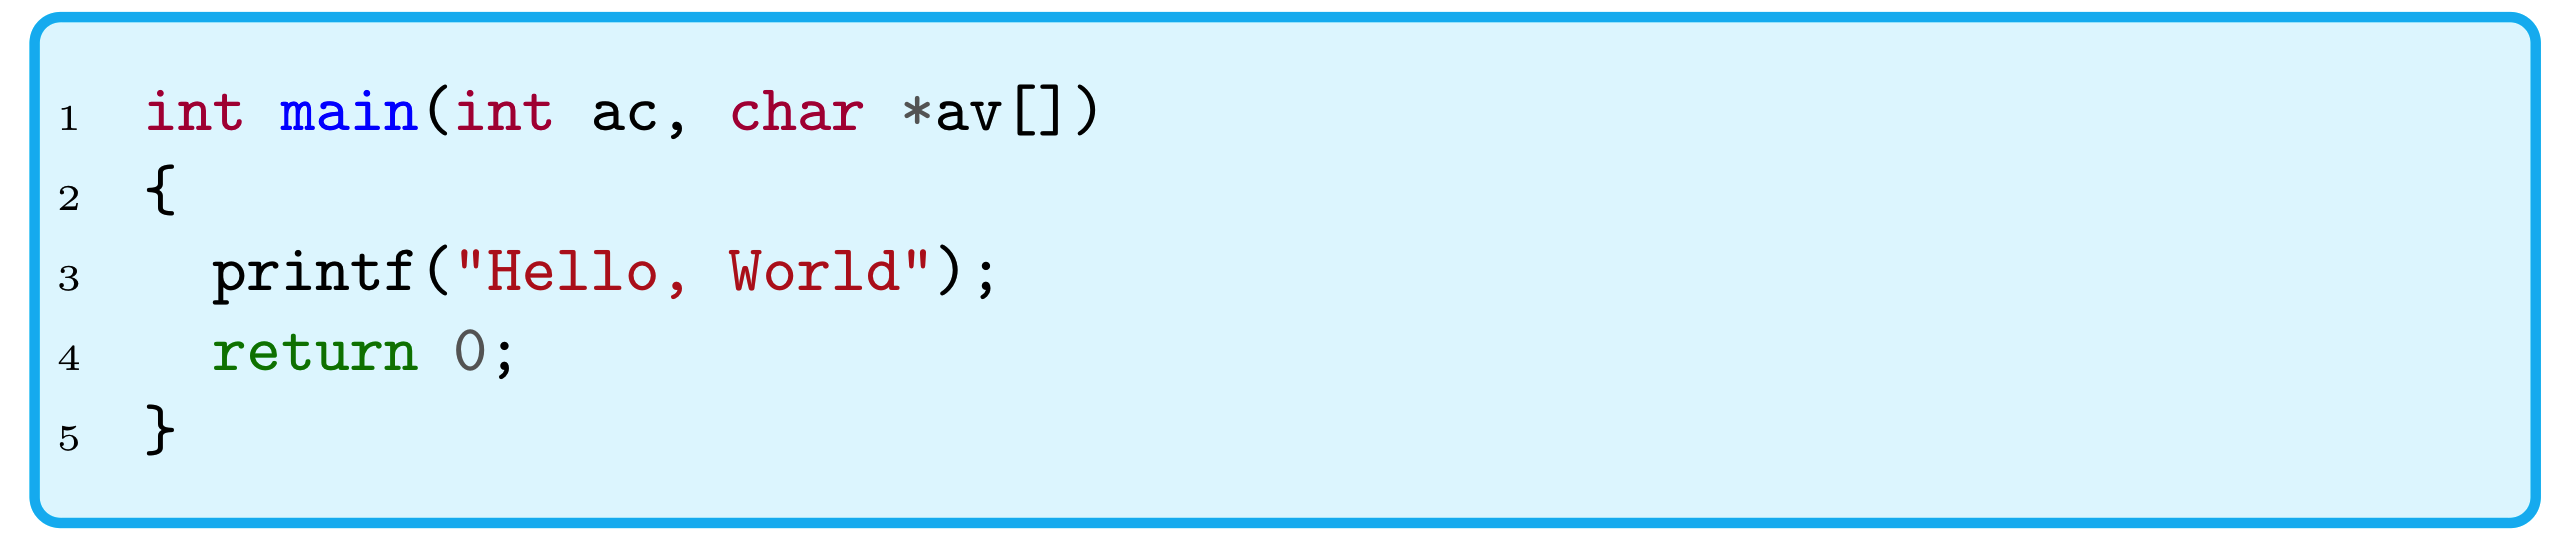
\includegraphics[width=1\linewidth]{3.4.png}} }{3.4}
\end{minipage}
&
\begin{minipage}[m]{0.55\textwidth}
\renewcommand\textminus{\mbox{-}}%<<<<<<<<<<<
\begin{lstlisting}[numberstyle=\zebra{pink!15}{green!15},numbers=left,basicstyle=\ttfamily\footnotesize] 
\documentclass{article}
\usepackage[many]{tcolorbox}
\tcbuselibrary{minted}
\newtcblisting{mylisting}{
  colframe=cyan,
  colback=cyan!10,
  listing only,
  listing engine=minted,
  minted language=cpp,
  minted options={fontsize=\small,linenos,numbersep=3mm},
}

\begin{document}
\begin{mylisting}
some code 
\end{mylisting}
\end{document}
\end{lstlisting}
\end{minipage}
\end{tabular}
\end{table}
%\enum{\href{https://tex.stackexchange.com/questions/670255/remove-thin-black-frame-around-standalone-image/670257#670257}{%}{3.5}
%-------------------3.5
\subsection{\hll{Run LaTeX code inside and show result}}
\begin{table}[h!]
\begin{tabular}{c | c}
\begin{minipage}[m]{0.4\textwidth}
\begin{tikzpicture}
\node (0,0) {\begin{minipage}[m]{0.90\textwidth}
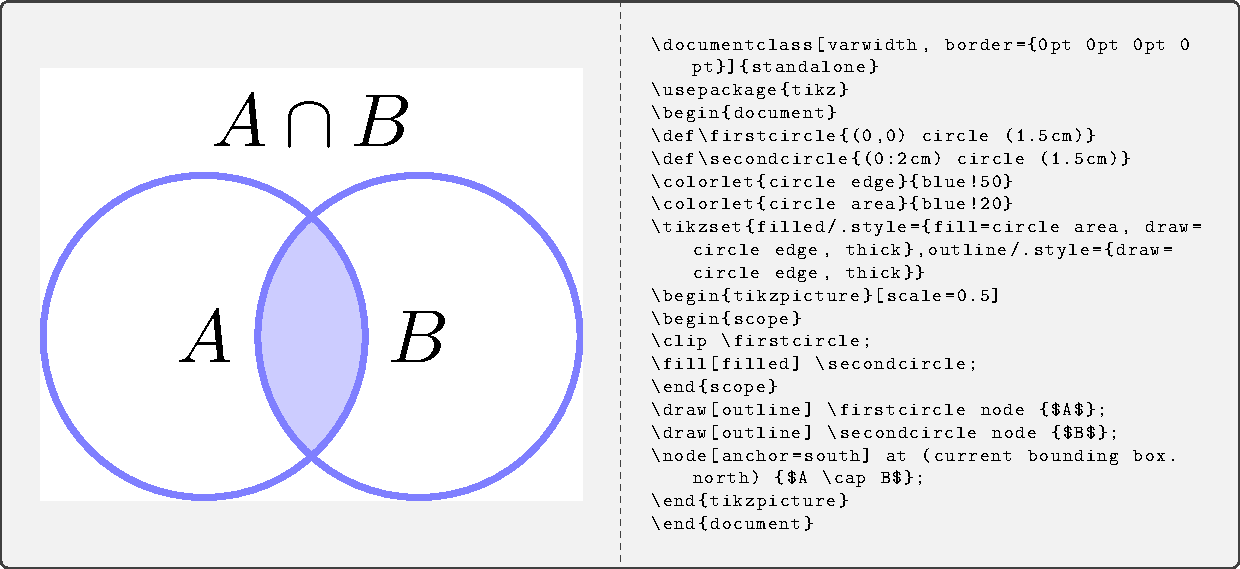
\includegraphics[width=1\linewidth]{C:/Users/user/Desktop/eBook/images/3.5.pdf}
\end{minipage} };
\node [opacity=0.05] (0,0) {\scalebox{8.0}{\textcolor{red}{\emph{3.5}}}};
\end{tikzpicture}
\end{minipage}
&
\begin{minipage}[m]{0.55\textwidth}
\renewcommand\textminus{\mbox{-}}%<<<<<<<<<<<
\begin{lstlisting}[numberstyle=\zebra{pink!15}{green!15},numbers=left,basicstyle=\ttfamily\footnotesize] 
\documentclass{standalone}
\usepackage[most]{tcolorbox}
\tcbset{sidebyside,width = 21cm,listing options={basicstyle=\small\ttfamily,breaklines=true}}
 
\begin{document}
\begin{tcblisting}{comment and listing, pdf comment, freeze pdf, compilable listing, run pdflatex, comment style={frame hidden,scale=2}}
\documentclass[varwidth, border={0pt 0pt 0pt 0pt}]{standalone}
\usepackage{tikz}
\begin{document}
\def\firstcircle{(0,0) circle (1.5cm)}
\def\secondcircle{(0:2cm) circle (1.5cm)}
\colorlet{circle edge}{blue!50}
\colorlet{circle area}{blue!20}
\tikzset{filled/.style={fill=circle area, draw=circle edge, thick},outline/.style={draw=circle edge, thick}}
\begin{tikzpicture}[scale=0.5]
\begin{scope}
\clip \firstcircle;
\fill[filled] \secondcircle;
\end{scope}
\draw[outline] \firstcircle node {$A$};
\draw[outline] \secondcircle node {$B$};
\node[anchor=south] at (current bounding box.north) {$A \cap B$};
\end{tikzpicture}
\end{document}
\end{tcblisting}
\end{document}
\end{lstlisting}
\end{minipage}
\end{tabular}
\end{table}

%-------------------3.6
\subsection{\hll{Breaking code lines in a tcolorbox}}
\begin{tabular}{l | c}
\begin{minipage}[m]{0.4\textwidth}
\begin{tikzpicture}
\node (0,0) {\begin{minipage}[m]{0.90\textwidth}
\begin{tcblisting}{colback=white,colframe=white,comment style={frame hidden,scale=2.5}, comment only, pdf comment, freeze pdf, compilable listing, run pdflatex,}
\documentclass[varwidth, border={10pt 10pt 10pt 10pt}]{standalone}
\usepackage{hyperref}
\usepackage[table]{xcolor}
\usepackage{listings}
\usepackage[most]{tcolorbox}
\usepackage{inconsolata}
\usepackage{graphicx}
\tcbuselibrary{breakable}

\newtcblisting[auto counter,number within=chapter]{sourcecode}[2][]{sharp corners, breakable,
    fonttitle=\bfseries, colframe=gray, listing only, 
    listing options={basicstyle=\ttfamily,language=php, showstringspaces=false, 
    breaklines=true, postbreak={\raisebox{0ex}[0ex][0ex]{\ensuremath{\color{red}\hookrightarrow\space}}}, tabsize=4
  }, 
    title=Code Snippet \thetcbcounter: #2, #1}


\begin{document}

\begin{sourcecode}{}
    <?php

    function abc($file_name){

        header('Content-Type: application/vnd.openxmlformats-officedocument.spreadsheetml.sheet');
        header('Content-Disposition: attachment;filename="'.$file_name.'"');
        header('Cache-Control: max-age=0');
        $writer->save('php://output');
    }

\end{sourcecode}

\end{document}
\end{tcblisting}
\end{minipage}};
\node [opacity=0.05] (0,0) {\scalebox{8.0}{\textcolor{red}{3.6}}};
\end{tikzpicture}
\end{minipage} 
&
\begin{minipage}[m]{0.55\textwidth}
\begin{lstlisting}[numberstyle=\zebra{black!5}{blue!15},numbers=left,basicstyle=\ttfamily\footnotesize] 
\documentclass{book}
\usepackage{hyperref}
\usepackage[table]{xcolor}
\usepackage{listings}
\usepackage[most]{tcolorbox}
\usepackage{inconsolata}
\usepackage{graphicx}
\tcbuselibrary{breakable}

\newtcblisting[auto counter,number within=chapter]{sourcecode}[2][]{sharp corners, breakable,
    fonttitle=\bfseries, colframe=gray, listing only, 
    listing options={basicstyle=\ttfamily,language=php, showstringspaces=false, 
    breaklines=true, postbreak={\raisebox{0ex}[0ex][0ex]{\ensuremath{\color{red}\hookrightarrow\space}}}, tabsize=4
  }, title=Code Snippet \thetcbcounter: #2, #1}

\begin{document}
\begin{sourcecode}{}
<?php

function abc($file_name){

header('Content-Type: application/vnd.openxmlformats-officedocument.spreadsheetml.sheet');
header('Content-Disposition: attachment;filename="'.$file_name.'"');
header('Cache-Control: max-age=0');
$writer->save('php://output');
}
\end{sourcecode}
\end{document}
\end{lstlisting}
\end{minipage}
\end{tabular}

%-------------------3.7
%https://tex.stackexchange.com/questions/452150/advanced-customization-of-minted-code
\subsection{\hll{Modern code listing using \xmyboxg{minted}}}
\begin{table}[h!]
\begin{tabular}{c | c}
\begin{minipage}[m]{0.4\textwidth}

paraiso-dark
\begin{javalst}
public class ClassName {
        public static void main(String[] args) {
            System.out.println(args);
        }
}
\end{javalst}
emacs
\begin{javalstt}
public class ClassName {
        public static void main(String[] args) {
            System.out.println(args);
        }
}
\end{javalstt}
vim
\begin{javalsttt}
public class ClassName {
        public static void main(String[] args) {
            System.out.println(args);
        }
}
\end{javalsttt} 
perldoc
\begin{javalstttt}
public class ClassName {
        public static void main(String[] args) {
            System.out.println(args);
        }
}
\end{javalstttt}
monokai
\begin{python}
public class ClassName {
        public static void main(String[] args) {
            System.out.println(args);
        }
}
\end{python}
\end{minipage}
&
\begin{minipage}[m]{0.55\textwidth}
\renewcommand\textminus{\mbox{-}}%<<<<<<<<<<<
\begin{lstlisting}[numberstyle=\zebra{pink!15}{green!15},numbers=left,basicstyle=\ttfamily\footnotesize]{tex}
\documentclass{article}
\usepackage[T1]{fontenc}
\usepackage{listings}
\usepackage{minted}
\usepackage{xcolor}
\usepackage{tcolorbox}
\tcbuselibrary{listings, minted, skins}
\tcbset{listing engine=minted}
\newtcblisting{javalst}{listing only, minted language=java, minted style=paraiso-dark,
    colback=bg, enhanced, frame hidden, minted options={fontfamily=fdm, 
    fontsize=\footnotesize, tabsize=2, breaklines, autogobble}}
\definecolor{inline}{RGB}{187,57,82}
\definecolor{bg}{RGB}{22,43,58}
\setminted[java]{bgcolor=bg, fontfamily=fdm, fontsize=\footnotesize}

\begin{document}
\begin{javalst}
    public class ClassName {
            public static void main(String[] args) {
                System.out.println(args);
            }
    }
\end{javalst}
\end{document}
\end{lstlisting}

For lines numbering (last example):

\begin{lstlisting}[numberstyle=\zebra{pink!15}{red!15},numbers=left,basicstyle=\ttfamily\scriptsize]{tex}
\documentclass{article}
\usepackage[T1]{fontenc}
\usepackage{listings}
\usepackage{minted}
\usepackage{xcolor}
\usepackage{tcolorbox}
\tcbuselibrary{listings, minted, skins}
\tcbset{listing engine=minted}
\renewcommand{\theFancyVerbLine}{\textcolor[rgb]{1,1,1}{\texttt\footnotesize\arabic{FancyVerbLine}}}
\newtcblisting{javalst}{listing only, minted language=java, minted style=paraiso-dark, colback=bg, enhanced,frame hidden,
minted options={fontsize=\footnotesize, tabsize=2, breaklines, autogobble, linenos, numbersep=5pt,fontsize=\small,},
overlay={\begin{tcbclipinterior}\fill[bg](frame.south west)rectangle([xshift=5mm]frame.north west);\end{tcbclipinterior}}}
\definecolor{inline}{RGB}{187,57,82}
\definecolor{bg}{RGB}{22,43,58}
\setminted[java]{bgcolor=bg, fontfamily=fdm, fontsize=\footnotesize}

\begin{document}
\begin{javalst}
    public class ClassName {
            public static void main(String[] args) {
                System.out.println(args);
            }
    }
\end{javalst}
\end{document}
\end{lstlisting}
\end{minipage}
\end{tabular}
\end{table}

%-------------------3.8
%-------------------3.9
%-------------------3.10








